\documentclass[fr]{../../../../../../eplexam}
\usepackage{amsmath,amssymb,amsthm}
\usepackage{tikz}
\usepackage{pgfplots}
\usetikzlibrary{datavisualization}
\usetikzlibrary{datavisualization.formats.functions}
\pgfplotsset{compat=1.15}

\DeclareMathOperator{\Res}{Res}

\hypertitle{Mathématiques}{3}{FSAB}{1103}{2018}{Janvier}{All}
{Martin Braquet \and Maxime Clément \and Guillaume Prieur \and Jean-Martin Vlaeminck}
{Jean-François Remacle, Grégoire Winckelmans et Roland Keunings}

\section{EDP-Q1}
On donne l'équation de transport sous forme conservative :
\[
    \fpart{(cu)}{x} + \fpart{u}{t} = S
\]
avec $$c = c(x) = \frac{c_0}{\cosh{\left(\frac{x}{L}\right)}}$$ où $c_0$ et $L$ sont des constantes.

Les conditions sont :
\begin{itemize} 
    \item Région A : $u(s, 0) = Ue^{-s/L_0}$ pour $s \geq 0$, où $U$ et $L_0$ sont des constantes.
    \item Région B : $u(0, \tau) = U$ pour $\tau \geq 0$.
\end{itemize}
\begin{enumerate}
	\item Obtenez les équations des caractéristiques
	pour la région A du quart de plan (c-à-d relation entre $s$, $x$ et $t$)
	et pour la région B (c-à-d relation entre $\tau$, $x$ et $t$).

	Faire une esquisse (propre avec des axes chiffrés !) des courbes caractéristiques
	qui émanent de $\frac{s}{L} = 0$, $\frac{s}{L} = 1$ et de $\frac{c_0\tau}{L} = 1$.
	Les deux régions doivent être clairement reconnaissables.

	\item Obtenez l'EDO à résoudre pour trouver l'évolution de $cu$
	le long de chaque caractéristique pour le cas $S$ général.

	Enfin, trouvez la solution  $u(x, t)$ dans la région $A$
	pour le cas particulier $S = c_0\frac{U}{L}$.
\end{enumerate}

Aide: $\cosh(0)=1$, $ \cosh(1)\simeq1.54$, $\cosh(2)\simeq3.76$,
$\int\cosh(a\eta)\mathrm{d}\eta=\frac{1}{a}\sinh(a\eta)$
et $\int\frac{\mathrm{d}\eta}{\cosh(a\eta)}=\frac{2}{a}\arctan(e^{a\eta})$.

\begin{solution}
\begin{enumerate}
	\item En développant l'équation, on obtient
	\[ c \fpart{u}{x} + \fpart{u}{t} = S - \fdif{c}{x} u \]
	qui permet d'identifier $P=c$, $Q=1$ et $R=S-\fdif{c}{x} u$.
	Par la relation de Laplace-Charpit,
	\begin{align*}
	P \dif{t} &= Q \dif{x} \\
	c \dif{t} &= \dif{x} \\
	\dif{t} &= \frac{1}{c} \dif{x} = \frac{1}{c_0} \cosh\left(\frac{x}{L}\right) \dif{x}.
	\end{align*}

	Pour la région A,
	\begin{align*}
	\int_{0}^{t} \dif{t'} &= \int_{s}^{x} \frac{1}{c_0} \cosh\left(\frac{x'}{L}\right) \dif{x'} \\
	t &= \frac{L}{c_0} \left[\sinh\left(\frac{x'}{L}\right)\right]_{s}^{x} \\
	&= \frac{L}{c_0} \left(\sinh(x/L) - \sinh(s/L)\right)
	\end{align*}
	ce qui permet de tracer $t$ en fonction de $x$ pour une caractéristique $s$ donnée,
	et aussi d'obtenir $s$:
	\[ s = L \cdot \arcsinh\left( \sinh\left(\frac{x}{L}\right) - \frac{c_0 t}{L} \right) \]

	Pour la région B,
	\begin{align*}
	\int_{\tau}^{t} \dif{t'} &= \int_{0}^{x} \frac{1}{c(x')} \dif{x'} \\
	t-\tau &= \frac{L}{c_0} \sinh\left(\frac{x}{L}\right) \\
	t &= \tau + \frac{L}{c_0} \sinh\left(\frac{x}{L}\right) \\
	\tau &= t - \frac{L}{c_0} \sinh\left(\frac{x}{L}\right).
	\end{align*}

	Pour tracer ces graphes, il faut se rappeler que pour des valeurs de $x$ assez grandes ($>1.15$),
	la fonction $\sinh(x)$ s'approche fortement d'une exponentielle (à 10\% près).
	Pour des valeurs de $x$ petites, la fonction tend à se diriger vers l'origine selon une droite.

	\begin{solfig}{q1_characts}{Réseau de caractéristiques de la question 1}
%		%\pgfdeclaredataformat{}
%		\begin{tikzpicture}
%		\datavisualization[
%			scientific axes=clean,
%			x axis={label=$x/L$},
%			y axis={label=$c_0t/L$},
%			visualize as smooth line/.list={0, 1, 2, 3},
%			style sheet=strong colors,
%			%regA={label in legend={text=regionA}},
%			%regB={label in legend={text=regionB}},
%			data/format=function
%		]
%		data [set=regA] {
%			var set : {0, 1, 2, 3};%interval[0:3] step 1;
%			var x : interval[0:3] samples 20;
%			%var x : interval[\value{set}:3] samples 20;
%			func y = sinh(\value x) - sinh(\value{set});
%		}
%%		data [set=regB] {
%%			var t : interval[0:5] step 1;
%%			var x : interval[0:3] samples 20;
%%			func y = \value{t} + sinh(\value x);
%%		}
%		;
%		\end{tikzpicture}
		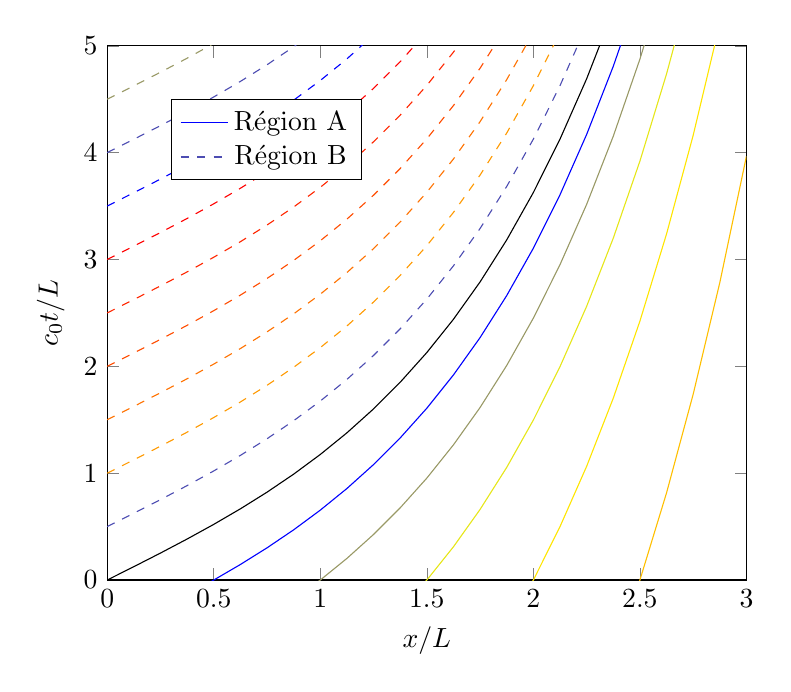
\begin{tikzpicture}
		\begin{axis}[
			xlabel=$x/L$,
			ylabel=$c_0t/L$,
			ymin=0,
			ymax=5,
			xmin=0,
			xmax=3,
			width=0.8\textwidth,
			colormap name=hot,
			cycle list={
				[colors of colormap={0, 100, ..., 1000}]
			},
			legend style={at={(0.1, 0.9)}, anchor=north west},
			%cycle from colormap manual style,
		]
		\addplot+[mark=none, domain=0:3, forget plot, color=black] {sinh(x)};
		\addplot+[mark=none, domain=0:3] {sinh(x)-sinh(0.5)};
		\addplot+[mark=none, domain=0:3, dashed] {0.5+sinh(x)};
		\foreach \s in {1, 1.5, ..., 2.5}{
			\addplot+[mark=none, domain=0:3] {sinh(x) - sinh(\s)};
		}
		\foreach \t in {1, 1.5, ..., 4.5}{
			\addplot+[mark=none, domain=0:3, dashed] {\t+sinh(x)};
		}
		\legend{Région A, Région B};
		\end{axis}
		\end{tikzpicture}
	\end{solfig}
	La figure~\ref{fig:q1_characts} montre les caractéristiques dans le quart de plan.
	La région A est à droite de la caractéristique passant par l'origine, la région B à gauche.

	\item Pour résoudre l'équation avec la méthode traditionnelle,
	il nous faut déterminer $u$ grâce aux relations de compatibilité
	(les autres associations de terme dans $\frac{\dif{x}}{P} = \frac{\dif{t}}{Q} = \frac{\dif{u}}{R}$).
	La relation de compatibilité nous donne
	\begin{align*}
	P \dif{u} &= R \dif{x} \\
	c(x) \dif{u} &= \left( S - \fdif{c}{x} u \right) \dif{x}
	\end{align*}
	avec $\fdif{c}{x} = - \frac{c_0}{L} \frac{\sinh(x/L)}{\cosh^2(x/L)}$.

	Cette relation a l'air déjà peu agréable, et elle le devient d'autant plus
	lorsqu'on cherche à résoudre l'équation pour le cas spécial $S=\frac{c_0 U}{L}$.
	En effet, la relation devient alors
	\[ c(x) \dif{u} = \frac{c_0 U}{L} \dif{x} - \frac{c_0}{L} \frac{\sinh(x/L)}{\cosh^2(x/L)} u \dif{x} \]
	et on voit mal comment on va séparer les variables dans cette relation.

	A la place, autant bien lire les consignes et remarquer qu'on nous demande de trouver une relation pour $cu$, et non pour $u$.
	L'étudiant attentif et ayant lu son syllabus se souviendra que
	dans le cas de l'équation de transport sous forme conservative $\fpart{(c(x) u)}{x} + \fpart{u}{t} = 0$,
	le terme $cu$ est en fait constant le long des caractéristiques.
	Ici, on n'a pas exactement l'équation de transport du syllabus\footnote{Ce serait probablement trop simple pour un examen,
		se disent les professeurs.}, mais on peut quand même trouver quelque chose:
	\begin{align*}
	c(x) \dif{u} &= S \dif{x} - u \fdif{c}{x} \dif{x} \\
	c(x) \dif{u} + u \dif{c(x)} &= S \dif{x} \\
	\dif{(cu)} &= S \dif{x}.
	\end{align*}
	Le passage de $\fdif{c}{x} \dif{x}$ à $\dif{c}$ se comprend mieux lorsqu'on l'effectue dans l'autre sens,
	et qu'on se rappelle de ce qu'est une différentielle.

	Dès lors, nous avons une relation pratique pour déterminer $u$ partout
	(pour peu que $S$ ne dépende pas de $u$ évidemment; sinon on est de retour
	aux problèmes précédents, et forcé d'utiliser des méthodes numériques)
	\[ \dif{(cu)} = S \dif{x} \]

	Appliquons-là au cas spécial $S=\frac{c_0 U}{L}$:
	\begin{align*}
	\int_{(s, 0)}^{(x, t)} \dif{(cu)} &= \frac{c_0 U}{L} \int_{s}^{x} \dif{x} \\
	c(x) u(x, t) - c(s) u(s, 0) &= c_0 U \frac{x-s}{L} \\
	c(x) u(x, t) &= c(s) u(s, 0) + c_0 \frac{x-s}{L} U \\
	u(x, t) &= \frac{c(s)}{c(x)} u(s, 0) + \frac{c_0}{c(x)} \frac{x-s}{L} U
	\end{align*}
	ce qui donne finalement
	\[
	  u(x, t) = U \frac{\cosh\left(\frac{x}{L}\right)}{\cosh\left(\frac{s(x, t)}{L}\right)} \exp\left( -\frac{s(x, t)}{L_0} \right)
	    + U \cosh\left(\frac{x}{L}\right) \frac{x-s(x, t)}{L},
	\]
	% Ancien développement, gardé pour raisons historiques (autant garder les calculs)
%	\begin{align*}
%	s &= L \cdot \arcsinh\left( \sinh\left(\frac{x}{L}\right) - \frac{c_0 t}{L} \right) \\
%	u(s, 0) &= U \exp\left( -\frac{s}{L_0} \right) \\
%	\end{align*}
%	en posant $k(x, t) = \sinh\left(\frac{x}{L}\right) - \frac{c_0 t}{L}$, on obtient après calculs
%	\begin{align*}
%	c(s) &= \frac{c_0}{\sqrt{1 + k(x, t)^2}} \\
%	e^{-s/L} &= \frac{1}{k(x, t) + \sqrt{1+k(x, t)^2}} \\
%	e^{-s/L_0} &= \left(e^{-s/L}\right)^{L/L_0} \\
%	\end{align*}
%	ce qui donne, une fois injectés dans l'expression de $u$,
%	\begin{equation}
%	u(x, t) = \frac{ \cosh\left( \frac{x}{L} \right) }{ \sqrt{ 1 + k(x, t)^2} } \frac{1}{\left( k(x, t) + \sqrt{k(x, t)^2 + 1} \right)^{L/L_0}} U
%	           + \cosh\left(\frac{x}{L}\right) \frac{x - s}{L} U
%	\end{equation}
	une belle solution complexe comme on les aime.

	Pour être complet, voici la solution pour la région B:
	\[ u(x, t) = U \cosh\left( \frac{x}{L} \right) \left( 1 + \frac{x}{L} \right). \]

	La question était nettement plus compliquée que l'examen de août 2017,
	qui était aussi une équation de transport. Ici, la complexité des fonctions hyperboliques
	combinée au choix de $S$ et à la double condition limite dans deux régions différentes
	n'aidait pas à obtenir une solution facile.
\end{enumerate}
\end{solution}

\section{EDP-Q2}
On considère l'équation de Laplace
\[
    \nabla^2 u = \frac{\partial^2 u}{\partial x^2}+\frac{\partial^2 u}{\partial y^2} = 0
\]
à l'intérieur d'un rectangle tel que $0\leq x\leq L$ et $0\leq y \leq H$.
 
Les conditions limites sont:
\[
 u(0, y) = 0 ,\qquad u(L, y) = U \frac{y}{H} ,\qquad u(x, 0) = 0 \qquad \mathrm{et} \qquad \fpart{u}{y}(x, H) =\frac{U}{H} f\left(\frac{x}{L}\right).
\]
\begin{enumerate}
\item
Il est demandé de résoudre cette équation pour le cas $f\left(\frac{x}{L}\right)$ général,
en utilisant \textbf{une seule fois la séparation de variables}.
(\textbf{Aide:} utiliser le mode 0, $u_0(x,y) = U\frac{x}{L}\frac{y}{H}$, et une superposition).
Veillez à écrire clairement les intégrales à devoir finalement effectuer
pour obtenir les coefficients du développement en série de la solution.
\item Obtenez ensuite la solution détaillée pour le cas particulier $f\left(\frac{x}{L}\right) = \sin\left(2\pi \frac{x}{L}\right) + \frac{x}{L}$.
\end{enumerate}


\begin{solution}

Le rectangle est représenté comme suit
\begin{center}
    \begin{tikzpicture}
      \draw[->] (0,0) -- (3,0) node[right] {$x$};
      \draw[->] (0,0) -- (0,2.25) node[above] {$y$};
      \draw[-] (2.25,0) -- (2.25,1.5);
      \draw[-] (0,1.5) -- (2.25,1.5);
      \put(-12.5, 20){$1$}
      \put(30, 47.5){$2$}
      \put(70, 20){$3$}
      \put(30, -12.5){$4$}
      \put(60, -12.5){$L$}
      \put(-12.5, 40){$H$}
    \end{tikzpicture}
\end{center}
Les conditions sur les bords sont
\begin{enumerate}
    \item $u(0,y) = 0$
    \item $\frac{\partial u }{\partial y}(x,H) =\frac{U}{H} f\left(\frac{x}{L}\right)$
    \item $u(L, y) = U\frac{y}{H}$
    \item $u(x,0) = 0$
\end{enumerate}

Par séparation de variable, on écrit $u$ sous la forme
\[u(x,y) = X(x)Y(y)\]
On l'introduit dans l'EDP et on obtient
\begin{align*}
    & X'' + Y'' = 0\\
    & \frac{X''}{X} = -\frac{Y''}{Y} = \lambda
\end{align*}
On résout d'abord le mode $\lambda=0$ pour obtenir une solution particulière que nous noterons $u_0(x,y)$.
On obtient l'équation pour $X_0$
\[ X_0''(x) = 0 \]
qui a pour solution
\[ X_0(x) = Ax + B \]
et l'équation pour $Y_0$
\[ Y_0''(y) = 0 \]
qui a pour solution
\[ Y_0(y) = Cy + D \]
et donc la solution pour $u_0$ est de la forme
\[ u_0(x, y) = (Ax+B) (Cy+D) = (Ax+B) (y+ D'). \]
Par la condition en $x=0$ (1),
\[ u(0, y)=0 \implies X(0) = 0 \implies B = 0. \]
Par la condition en $y=0$ (4),
\[ u(x, 0)=0 \implies Y(0) = 0 \implies D' = 0. \]
Par la condition en $x=L$ (3),
\[ u(L, y) = A L y = U \frac{y}{H} \implies A = \frac{U}{L H}. \]
On a pour solution du mode zéro
\[ u_0(x, y) = U\frac{y}{H}\frac{x}{L} \]
comme annoncé dans l'énoncé.

Notons maintenant notre solution générale telle que 
\[ u(x, y) = u_g(x, y) + u_0(x, y). \]
On résout maintenant le mode $\lambda \neq 0$ pour obtenir cette solution générale.
Les conditions limites pour $u_g$ changent pour tenir compte de $u_0$; notamment,
\[ u_g(L, y) = u(L, y) - u_0(L, y) = 0, \]
et
\[ \fpart{u_g}{y}(x, H) = \fpart{u}{y}(x, H) - \fpart{u_0}{y}(x, H) = \frac{U}{H} \left(f\left(\frac{x}{L}\right) - \frac{x}{L}\right). \]
Au vu des conditions homogènes en $x$, on choisit $\lambda=-k^2$.
On obtient l'équation pour $X_g(x)$
\[ X_g''(x) = -k^2 X_g(x) \]
qui a pour solution
\[ X_g(x) = A\cos(kx) + B\sin(kx). \]
Par la condition homogène en $x=0$ nous avons
\[ X_g(0) = 0 \implies A=0. \]
Par la condition homogène en $x=L$ nous avons
\[ X_g(L) = 0 \implies B\sin(kL) = 0 \implies k_n = \frac{n\pi}{L} \qquad n = 1,2,3, \dots \]
ce qui permet de dire que $X_g(x) = B \sin(k_n x)$.
On prend $B=1$ sans perte de généralité.
On obtient l'équation pour $Y_{g,n}(y)$
\[ Y_{g,n}''(y) = k_n^2 Y_{g,n}(y) \]
qui a pour solution
\[ Y_{g,n}(y) = C_n\cosh(k_ny) + D_n\sinh(k_ny). \]
Par la condition sur le bord (4)
\[ u_{g, n}(x, 0) = 0 \implies Y_{g,n}(0) = 0 \implies C = 0. \]
Notre solution générale est donc donnée par 
\[ u_{g,n}(x,y) = D_n \sin(k_n x)\sinh(k_n y). \]
Par superposition des solutions, on a
\[ u_g(x,y) = \sum_{n=1}^\infty D_n \sin(k_n x)\sinh(k_n y). \]
On peut donc écrire la solution de notre équation en terme de $D_n$ à calculer
\begin{align*}
u(x, y) & = u_0(x, y) + \sum_{n=0}^\infty D_n\sin(k_nx)\sinh(k_ny) \\
& = U\frac{y}{H}\frac{x}{L} + \sum_{n=1}^\infty D_n\sin(k_nx)\sinh(k_ny) \qquad k_n=\frac{n\pi}{L}.
\end{align*}
Il reste la dernière condition sur le bord (2) pour déterminer les $D_n$.
\[
\fpart{u_g}{y}(x, H) = \sum_{n=1}^\infty \underbrace{D_n k_n \cosh(k_n H)}_{E_n} \sin(k_n x)
= \frac{U}{H} \left( f\left(\frac{x}{L}\right) - \frac{x}{L} \right).
\]
En multipliant de part et d'autre par $\sin(k_m x)$ et par orthogonalité des fonctions propres, on a
\[ D_n = \frac{2}{L} \frac{1}{k_n \cosh(k_n H)} \frac{U}{H} \int^L_0 \left[ f\left(\frac{x}{L}\right) - \frac{x}{L}\right] \sin(k_nx) \dif{x}. \]
Et la solution complète est
\[ u(x,y) = \frac{U}{HL}\left[xy
          + \sum_{n=1}^\infty
          2 \frac{L}{n\pi} \frac{\sinh(\frac{n\pi}{L}y)}{\cosh(\frac{n\pi}{L}H)}
          \sin\left(\frac{n\pi x}{L} \right)
          \int^L_0 \left( f\left(\frac{X}{L}\right) - \frac{X}{L} \right)
          \sin\left(\frac{n\pi x}{L}\right) \dif{x}
          \right]. \]

Pour le cas particulier qui nous intéresse,
\begin{align*}
D_n &= \frac{2}{L} \frac{1}{k_n \cosh(k_n H)} \frac{U}{H} \int^L_0 \left[ \sin\left(2 \pi \frac{x}{L}\right) + \frac{x}{L} - \frac{x}{L}\right] \sin(k_nx) \dif{x} \\
&= \frac{2}{L} \frac{1}{k_n \cosh(k_n H)} \frac{U}{H} \int^L_0 \sin\left(2 \pi \frac{x}{L}\right) \sin\left(\frac{n\pi x}{L}\right) \dif{x} \\
&= \begin{cases}
\frac{U}{H} \frac{1}{k_n \cosh(k_n H)} & \text{si } n=2 \\
0 & \text{sinon}
\end{cases}
\end{align*}
Finalement,
\[ u(x, y) = U \frac{x}{L} \frac{y}{H}
  + U \frac{L}{2H\pi}
    \frac{\sinh(\frac{2\pi y}{L})}{\cosh(\frac{2\pi H}{L})}
    \sin\left(\frac{2 \pi x}{L}\right)
\]
où on notera que le $2$ au dénominateur vient du $n=2$.


\end{solution}

\section{COMPLEXE-Q1}

On considère la fonction
\[
f(z) = g(z) e^{1/z}
\]
où $g(z)$ est une fonction entière.

\begin{enumerate}
    \item Calculez le résidu de la fonction en $z=0$.
    \item Donnez les points singuliers de la fonction $f$ et précisez leur type.
\end{enumerate}

\begin{solution}

\begin{enumerate}
\item
Développons la fonction $f(z)$ en série de Laurent
\begin{align*}
    e^z &= 1 + z + \frac{z^2}{2} + \frac{z^3}{6} + \dots = \sum_{n=0}^{\infty} \frac{1}{n!} z^n \\
    e^{1/z} &= 1 + \frac{1}{z} + \frac{1}{2z^2} + \frac{1}{6z^3} + \dots = \sum_{n=0}^{\infty} \frac{1}{n!} z^{-n}.
\end{align*}
La fonction $g(z)$ étant entière, nous pouvons, elle-aussi,
la développer en série de Taylor (donc de Laurent) autour de $z=0$:
\begin{equation*}
    g(z) = g(0) + g'(0)z + g''(0)\frac{z^2}{2} + \dots = \sum_{n=0}^{\infty} \frac{g^{(n)}(0)}{n!} z^n.
\end{equation*}
Il suffit à présent de multiplier les deux séries et d'en extraire le coefficient de $\frac{1}{z}$: 
\begin{align*}
    f(z) =& g(z) e^{1/z} \\
    =& \left(g(0) + g'(0)z + g''(0) \frac{z^2}{2} + \dots\right)
    \cdot \left(1 + \frac{1}{z} + \frac{1}{2z^2} + \frac{1}{6z^3} + \dots \right) \\
    =& \dots + \left( g'(0) + \frac{g''(0)}{2! \cdot 1!} + \frac{g'''(0)}{3! \cdot 2!} + \dots \right) z^{1} \\
    &+ \left(g(0) + g'(0)+ \frac{g''(0)}{(2!)^2} + \dots \right) z^0 \\
    &+ \left(\frac{g(0)}{0!\cdot 1!} + \frac{g'(0)}{1!\cdot 2!} + \frac{g''(0)}{2!\cdot 3!} + \dots \right) z^{-1} + \dots \\
    =& \sum_{k=-\infty}^{\infty} \left( \sum_{m=\min(k, 0)}^{\infty} \frac{1}{m!} \frac{1}{(m-k)!} g^{(m)}(0) \right) z^{k}.
\end{align*}
D'où on détermine le résidu:
\begin{equation*}
    \Res(f,0) = \sum_{n=0}^{\infty}\frac{g^{(n)}(0)}{n!(n+1)!}.
\end{equation*}

A noter que la double somme n'était clairement pas nécessaire à l'examen;
mais elle évite d'avoir à manipuler une double infinité de termes,
et rend les choses plus rigoureuses.

\item
La fonction $g(z)$ étant entière, c'est-à-dire définie partout,
le problème se ramène au calcul des points singuliers de la fonction $h(z) = e^{1/z}$.
Le seul point singulier est $z=0$. C'est un point singulier essentiel.
Pour plus de détails, voir l'examen de août 2017 ainsi que le syllabus du cours.

\end{enumerate}

\end{solution}

\section{COMPLEXE-Q2}

En utilisant le théorème des résidus, évaluez l'intégrale suivante:
\[
I = \int_0 ^{+\infty} \frac{x^{1/4}}{(x+1)(x+2)} \dif{x}.
\]
Veillez à bien justifier toutes les étapes de calcul.
Tous les lemmes de Jordan sont donnés.

\begin{solution}

Pour résoudre cette question, nous considérons la fonction
\begin{equation*}
    f(z) = \frac{z^{1/4}}{(z+1)(z+2)}
\end{equation*}
que nous intégrons sur un contour fermé en keyhole (ou pacman) dans le sens anti-horloger.
La fonction est multiforme, il faut donc effectuer une coupure avant de pouvoir intégrer.
L'unique point de branchement est $z=0$.
On décide, par conséquent, de faire une coupure telle que $0\leq\arg(\theta) < 2\pi$.
On observe aisément qu'il y a 2 pôles d'ordre 1 dans le contour; un en $z=-1$ et un en $z=-2$.
Nous pouvons d'ores et déjà calculer leur résidu:
\begin{align*}
    \Res(f, -1) &= \frac{z^{1/4}}{z+2}\bigg\rvert_{-1} = e^{\imag\frac{\pi}{4}} = \frac{\sqrt{2}}{2}(1+\imag)\\
    \Res(f, -2) &=\frac{z^{1/4}}{z+1}\bigg\rvert_{-2} = -2^{1/4}e^{\imag\frac{\pi}{4}} = -2^{-1/4}(1+\imag).
\end{align*}
Par le théorème des résidus on sait donc que:
\[ \oint_C f(z) dz = 2\imag\pi(2^{-1/2}-2^{-1/4})(1+\imag)
  = \pi(2^{1/2}-2^{3/4})(\imag-1). \]
Il reste à évaluer l'intégrale sur le keyhole. On peut la décomposer comme suit:
\begin{align*}
    \oint_C f(z)dz &= \underbrace{\int_\epsilon^R f(z)\dif{z}}_{I_1 = I}
     + \underbrace{\int_0^{2\pi - \delta} f\left( Re^{\imag\theta} \right) R \imag e^{\imag \theta} \dif{\theta}}_{I_2} \\
    &+ \underbrace{\int_R^\epsilon f\left(re^{(2\pi - \delta)\imag}\right) e^{(2\pi-\delta)\imag} \dif{r}}_{I_3}
     + \underbrace{\int_{2\pi - \delta}^0 f\left( \epsilon e^{\imag\theta} \right) \epsilon ie^{i\theta} \dif{\theta}}_{I_4}.
\end{align*}

La première intégrale est l'intégrale que l'on souhaite calculer,
lorsqu'on fait tendre $\epsilon$ vers $0$ et $R$ vers $\infty$.
Remarquons au passage que $f(z)$ n'a pas de bizarreries dans les parages de $0$ ou $\infty$
(des éventuels pôles ou points singuliers de la fonction),
et donc que $I$ est bien définie.

La seconde intégrale peut se résoudre avec le deuxième lemme de Jordan (celui avec $R\rightarrow\infty$).
En effet, en posant $z=R \e^{\imag \theta}$,
\[
  0 \le \abs{f(z) \cdot z}
  = \frac{\abs{R^{5/4} \e^{\imag 5\theta/4}}}{\abs{R \e^{\imag\theta} + 1} \abs{R \e^{\imag\theta} + 2}}
  \le \frac{R^{5/4}}{(R - 1) (R - 2)}
\]
où on utilise l'inégalité triangulaire pour le dénominateur,
et le fait que $\abs{e^{\imag \theta}} = 1$ et $\abs{ab}=\abs{a}\abs{b}$.
En faisant tendre $R$ vers l'infini:
\[ 0 \le \lim_{R=\abs{z} \rightarrow \infty} \abs{f(z) \cdot z}
     \le \lim_{R\rightarrow \infty} \frac{R^{5/4}}{(R-1)(R-2)}
       = \lim_{R \rightarrow \infty} R^{-3/4} = 0 \]
et donc, le lemme est applicable, et $I_2=0$.

La quatrième intégrale peut se résoudre avec le premier lemme de Jordan.
De manière semblable à $I_2$,
\[ 0 \le \abs{f(z) \cdot z} \le \dots \le \frac{\epsilon^{5/4}}{(\epsilon - 1) (\epsilon - 2)} \]
et, en faisant tendre $\epsilon$ vers $0$,
\[ 0 \le \lim_{\epsilon=\abs{z} \rightarrow 0} \abs{f(z) \cdot z}
     \le \lim_{\epsilon\rightarrow 0} \frac{\epsilon^{5/4}}{(\epsilon - 1) (\epsilon - 2)}
       = 0 \]
et donc, $I_4=0$.

Reste à calculer $I_3$. Celle-ci vaut
\begin{align*}
I_3 &= \lim_{\delta \rightarrow 0} \int_{\infty}^{0} f\left(r \e^{\imag (2\pi-\delta)}\right) \dif{r \e^{\imag (2\pi-\delta)}} \\
&= \lim_{\delta \rightarrow 0} \int_{\infty}^{0}
     \frac{
       \left(r \e^{\imag (2\pi-\delta)}\right)^{1/4}
     }{
       \left(r \e^{\imag (2\pi-\delta)} + 1\right) \left(r \e^{\imag (2\pi-\delta)} + 2\right)
     } \e^{\imag (2\pi-\delta)} \dif{r} \\
&= \lim_{\delta \rightarrow 0} \int_{\infty}^{0}
     \frac{r^{1/4} \e^{\imag (\pi/2 \, - \, \delta/4)}}
       {(r + 1) (r + 2)} 1 \dif{r} \\
&= \int_{\infty}^{0} \frac{\imag r^{1/4}}{(r + 1) (r + 2)} 1 \dif{r} \\
&= - \imag \int_{0}^{\infty} \frac{x^{1/4}}{(x + 1) (x + 2)} 1 \dif{x} \\
&= - \imag \cdot I.
\end{align*}
Justifications: lorsque $\delta \rightarrow 0$, coupure ou pas,
$\e^{\imag (2\pi - \delta)}$ s'approche de $1$ par définition.
La coupure n'a pas d'influence sur les arguments individuels utilisés ici,
mais a une influence lors de la détermination du chemin.

Enfin, on a donc
\begin{align*}
(1 - \imag) I &= \pi (\sqrt{2} - \sqrt[4]{8}) (\imag - 1) \\
\implies I &= \pi (\sqrt[4]{8} - \sqrt{2})
 = \pi \sqrt{2} (\sqrt[4]{2} - 1) \approx 0.840625.
\end{align*}

\end{solution}

\end{document}
